\documentclass[12pt,spanish]{article}
\usepackage[spanish]{babel}
\usepackage{tikz}
\usepackage{graphicx}
\usetikzlibrary{matrix,backgrounds,babel}
\usepackage{texdraw}
\usepackage{subcaption}
\usepackage{multirow}
\usepackage[hidelinks]{hyperref}
\usepackage{caption}
\usepackage{multicol}
\usepackage[outputdir=build]{minted}
\usepackage[skins,minted,breakable]{tcolorbox}
\usepackage{float}
\usepackage{array}
\graphicspath{ {../img/} {../../LaTeX/img/} {/home/csp98/latex/img/}}
\selectlanguage{spanish}
\usepackage[utf8]{inputenc}
\usepackage{graphicx}
\usepackage[a4paper,left=3cm,right=2cm,top=2.5cm,bottom=2.5cm]{geometry}
\newtheorem{ppio}{Principio }

\newmintedfile[cppcode]{c++}{
linenos=true,
breaklines=true,
tabsize=2,
}

\newmintedfile[script]{bash}{
linenos=true,
breaklines=true,
tabsize=2,
}

\makeindex

\begin{document}
\begin{titlepage}

\newlength{\centeroffset}
\setlength{\centeroffset}{-0.5\oddsidemargin}
\addtolength{\centeroffset}{0.5\evensidemargin}
\thispagestyle{empty}

\noindent\hspace*{\centeroffset}
\begin{minipage}{\textwidth}

\centering
\includegraphics[width=0.9\textwidth]{logo_ugr.jpg}\\[1.4cm]

\textsc{ \Large Algorítmica\\[0.2cm]}
\textsc{GRADO EN INGENIERÍA INFORMÁTICA}\\[1cm]

{\Huge\bfseries Práctica 3\\}
\noindent\rule[-1ex]{\textwidth}{3pt}\\[3.5ex]
{\large\bfseries El viajante de comercio}
\end{minipage}

\vspace{1.5cm}
\noindent\hspace*{\centeroffset}
\begin{minipage}{\textwidth}
\centering

\textbf{Autores}\\ {María Jesús López Salmerón \\ Nazaret Román Guerrero \\ Laura Hernández Muñoz \\ José Baena Cobos  \\ Carlos Sánchez Páez}\\[2.5ex]
\includegraphics[width=0.3\textwidth]{etsiit_logo.png}\\[0.1cm]
\vspace{1.5cm}
\includegraphics[width=0.5\textwidth]{decsai.jpg}\\[0.1cm]
\vspace{1cm}
\textsc{Escuela Técnica Superior de Ingenierías Informática y de Telecomunicación}\\
\vspace{1cm}
\textsc{Curso 2017-2018}
\end{minipage}
\end{titlepage}
\tableofcontents
\thispagestyle{empty}
\listoffigures
\newpage
\setcounter{page}{1}
%%%%%%%%%%%%%%%%%%%%%%%%Comienzo del documento%%%%%%%%%%%%%%%%%%%%%%%%%%%%%%%
\section{Descripción de la práctica}

El objetivo de esta práctica es abarcar el problema del viajante de comercio (TSP, \textit{Travel Salesman Problem}) mediante estrategias voraces. En concreto, seguiremos tres heurísticas diferentes:

\begin{enumerate}
	\item \textbf{Vecino más cercano}.
	\item \textbf{Inserción más económica}.
	\item \textbf{Derivado de Kruskal}.
\end{enumerate}

Todas las heurísticas desarrolladas tienen varias características en común:
\begin{itemize}
	\item \textbf{Conjunto de candidatos}. Ciudades a visitar.
	\item \textbf{Conjunto de seleccionados}. Aquellas ciudades que vayamos incorporando al circuito.
	\item \textbf{Función solución}. Todas las ciudades han sido visitadas y hemos vuelto a la primera.
	\item \textbf{Función de factibilidad}. La ciudad no ha sido visitada aún.
\end{itemize}

Por tanto, será la función de selección la que diferencie una de otra.

\section{Vecino más cercano}

\begin{itemize}
	\item \textbf{Función de selección}. Seleccionaremos aquella ciudad cuya distancia euclídea sea menor con respecto a la última ciudad añadida al conjunto de seleccionados.
\end{itemize}

Para abarcar más posibilidades, ejecutaremos el algoritmo voraz teniendo en cuenta todas las posibles ciudades de inicio, quedándonos con la distancia total más pequeña.

\section{Inserción más económica}

\begin{itemize}
	\item \textbf{Función de selección}. Seleccionamos la ciudad que incremente mínimamente la distancia total del circuito.
\end{itemize}

El conjunto de seleccionados comienza inicializado por el circuito formado por las ciudades más al norte, más al este y más al oeste.

\section{Derivado de Kruskal}

\begin{itemize}
	\item \textbf{Función de selección}. Elegiremos aquella arista cuyo coste sea menor y cuyas ciudades no hayan sido visitadas aún.
\end{itemize}

Si el número de ciudades es impar, forzosamente tendremos que añadir la ciudad faltante al final, justo antes de cerrar el circuito.


\section{Comparación de estrategias}

%Tabla con distancias y distancia óptima

\begin{figure}[H]
\centering
\begin{tabular}{|c|c|}
\hline
\multicolumn{2}{|c|}{\textit{ulysses16.tsp}}\\
\hline
\textbf{Vecino más cercano} & 77.1269\\
\textbf{Inserción más económica} & 51.9733\\
\textbf{Derivado de Kruskal} & \\
\textbf{Solución más óptima} & 74.1087\\
\hline
\end{tabular}
\vspace{0.5cm}
\quad
\begin{tabular}{|c|c|}
\hline	
\multicolumn{2}{|c|}{\textit{gr96.tsp}}\\
\hline
\textbf{Vecino más cercano} & 603.302\\
\textbf{Inserción más económica} & 620.367\\
\textbf{Derivado de Kruskal} & \\
\textbf{Solución más óptima} & 512.309\\
\hline	
\end{tabular}
\vspace{0.5cm}
\quad
\begin{tabular}{|c|c|}
\hline	
\multicolumn{2}{|c|}{\textit{a280.tsp}}\\
\hline
\textbf{Vecino más cercano} & 3094.28\\
\textbf{Inserción más económica} & 3192.42\\
\textbf{Derivado de Kruskal} & \\
\textbf{Solución más óptima} & 2586.77\\
\hline	
\end{tabular}
\vspace{0.5cm}
\quad
\begin{tabular}{|c|c|}
\hline	
\multicolumn{2}{|c|}{\textit{att48.tsp}}\\
\hline
\textbf{Vecino más cercano} & 39236.9\\
\textbf{Inserción más económica} & 40341.7\\
\textbf{Derivado de Kruskal} & \\
\textbf{Solución más óptima} & 33523.7\\
\hline	
\end{tabular}
\vspace{0.5cm}
\quad
\begin{tabular}{|c|c|}
\hline	
\multicolumn{2}{|c|}{\textit{pa561.tsp}}\\
\hline
\textbf{Vecino más cercano} & 18347\\
\textbf{Inserción más económica} & 17688.4 \\
\textbf{Derivado de Kruskal} & \\
\textbf{Solución más óptima} & 19330.8\\
\hline	
\end{tabular}
\vspace{0.5cm}
\quad
\begin{tabular}{|c|c|}
\hline	
\multicolumn{2}{|c|}{\textit{lin105.tsp}}\\
\hline
\textbf{Vecino más cercano} & 16939.4\\
\textbf{Inserción más económica} & 19063.7\\
\textbf{Derivado de Kruskal} & \\
\textbf{Solución más óptima} & 14383\\
\hline	
\end{tabular}
\vspace{0.5cm}
\quad
\begin{tabular}{|c|c|}
\hline	
\multicolumn{2}{|c|}{\textit{pr76.tsp}}\\
\hline
\textbf{Vecino más cercano} & 130921\\
\textbf{Inserción más económica} & 136636\\
\textbf{Derivado de Kruskal} & \\
\textbf{Solución más óptima} & 108159\\
\hline	
\end{tabular}
\vspace{0.5cm}
\quad
\begin{tabular}{|c|c|}
\hline	
\multicolumn{2}{|c|}{\textit{tsp225.tsp}}\\
\hline
\textbf{Vecino más cercano} & 4633.2\\
\textbf{Inserción más económica} & 4734.51\\
\textbf{Derivado de Kruskal} & \\
\textbf{Solución más óptima} & 3859 \\
\hline	
\end{tabular}
\vspace{0.5cm}
\quad
\begin{tabular}{|c|c|}
\hline	
\multicolumn{2}{|c|}{\textit{ch130.tsp}}\\
\hline
\textbf{Vecino más cercano} & 7198.74\\
\textbf{Inserción más económica} & 7455.72\\
\textbf{Derivado de Kruskal} & \\
\textbf{Solución más óptima} & 6110.86\\
\hline	
\end{tabular}
\vspace{0.5cm}
\quad
\begin{tabular}{|c|c|}
\hline	
\multicolumn{2}{|c|}{\textit{berlin52.tsp}}\\
\hline
\textbf{Vecino más cercano} & 8182.19\\
\textbf{Inserción más económica} & 9064.04\\
\textbf{Derivado de Kruskal} & \\
\textbf{Solución más óptima} & 7544.37\\
\hline	
\end{tabular}
\vspace{0.5cm}
\quad
\begin{tabular}{|c|c|}
\hline	
\multicolumn{2}{|c|}{\textit{rd100.tsp}}\\
\hline
\textbf{Vecino más cercano} & 9427.33\\
\textbf{Inserción más económica} & 9655.6\\
\textbf{Derivado de Kruskal} & \\
\textbf{Solución más óptima} & 9724.75\\
\hline	
\end{tabular}
\vspace{0.5cm}
\quad
\begin{tabular}{|c|c|}
\hline	
\multicolumn{2}{|c|}{\textit{st70.tsp}}\\
\hline
\textbf{Vecino más cercano} & 761.689\\
\textbf{Inserción más económica} & 824.228\\
\textbf{Derivado de Kruskal} & \\
\textbf{Solución más óptima} & 678.597 \\
\hline	
\end{tabular}
\caption{Comparación de resultados.}
\end{figure}

%figure con subfigures de los recorridos.
%%%%%%%%%%%%%%%%%%%%%%%
\begin{figure}[H]
\centering
\begin{subfigure}[b]{0.36\textwidth}
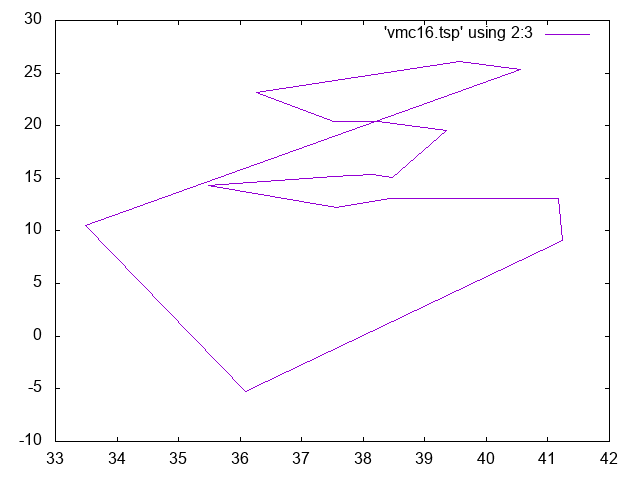
\includegraphics[width=\textwidth]{ulysses16_vmc.png}
\caption{Vecino más cercano}
\end{subfigure}
\quad
\begin{subfigure}[b]{0.36\textwidth}
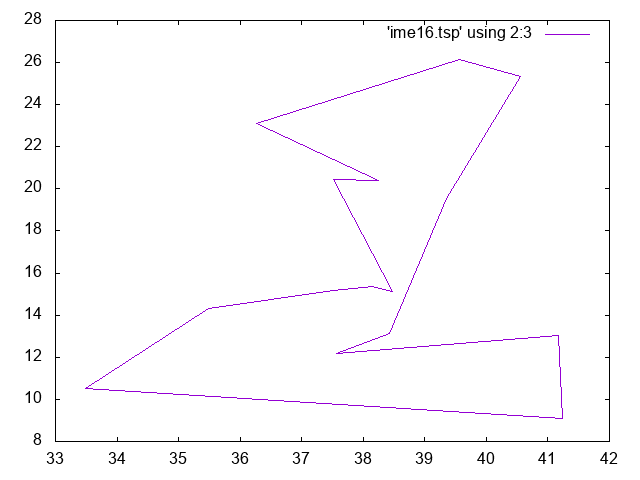
\includegraphics[width=\textwidth]{ulysses16_ime.png}
\caption{Inserción más económica}
\end{subfigure}

\vspace{1cm}

\begin{subfigure}[b]{0.36\textwidth}
%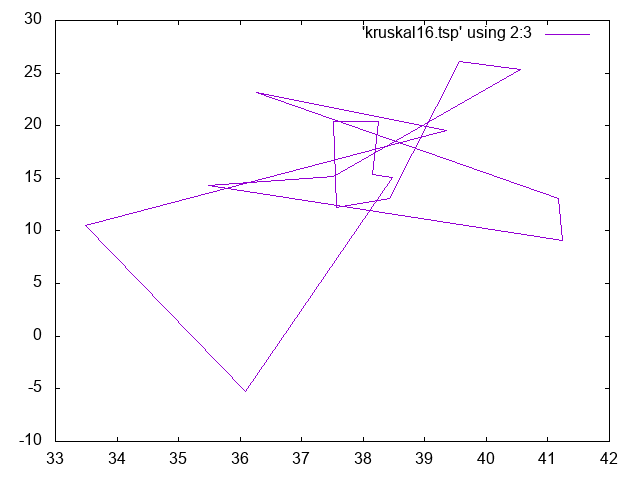
\includegraphics[width=\textwidth]{ulysses16_kruskal.png}
\caption{Derivado de Kruskal}
\end{subfigure}
\quad
\begin{subfigure}[b]{0.36\textwidth}
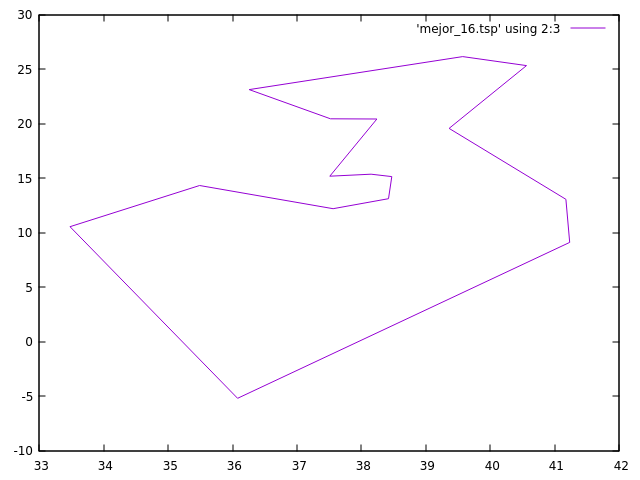
\includegraphics[width=\textwidth]{ulysses16_mejor.png}
\caption{Versión óptima}
\end{subfigure}
\caption{\textit{ulysses16.tsp}}
\end{figure}
%%%%%%%%%%%%%%%%%%%%%%%%%%%
\begin{figure}[H]
\centering
\begin{subfigure}[b]{0.36\textwidth}
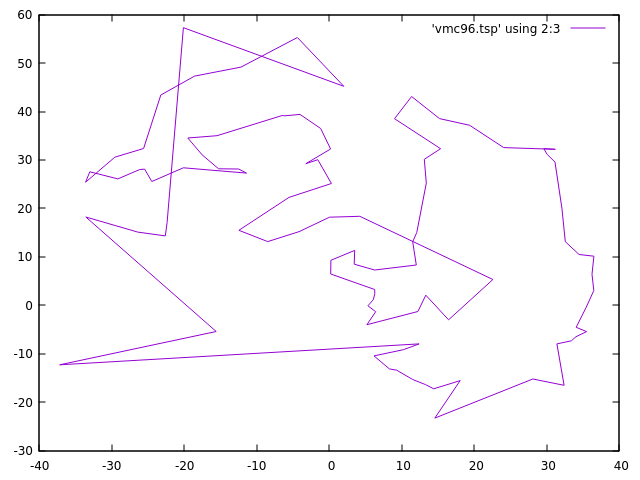
\includegraphics[width=\textwidth]{gr96_vmc.png}
\caption{Vecino más cercano}
\end{subfigure}
\quad
\begin{subfigure}[b]{0.36\textwidth}
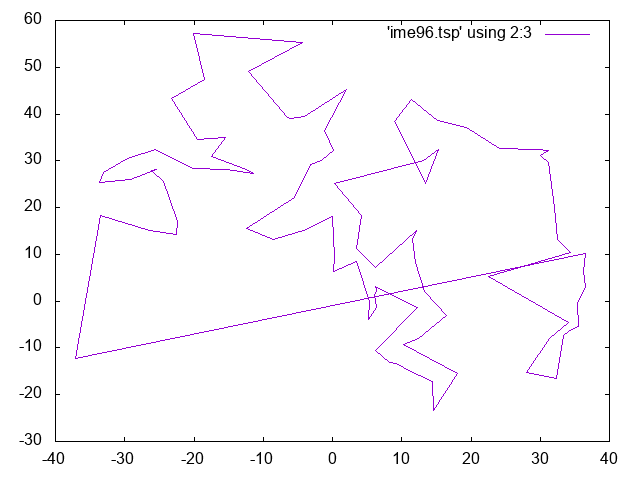
\includegraphics[width=\textwidth]{gr96_ime.png}
\caption{Inserción más económica}
\end{subfigure}

\vspace{1cm}

\begin{subfigure}[b]{0.36\textwidth}
%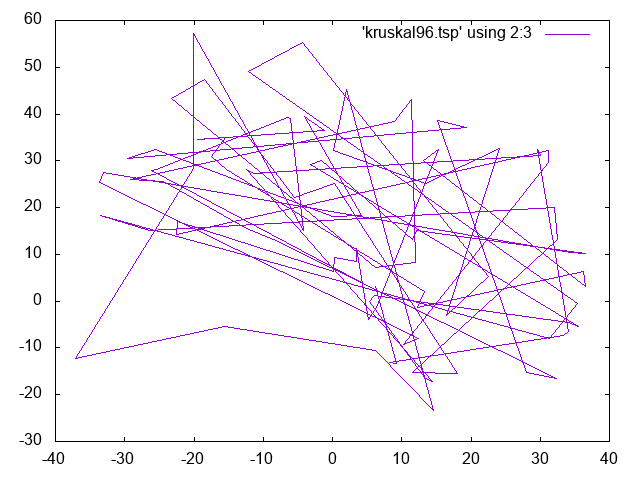
\includegraphics[width=\textwidth]{gr96_kruskal.png}
\caption{Derivado de Kruskal}
\end{subfigure}
\quad
\begin{subfigure}[b]{0.36\textwidth}
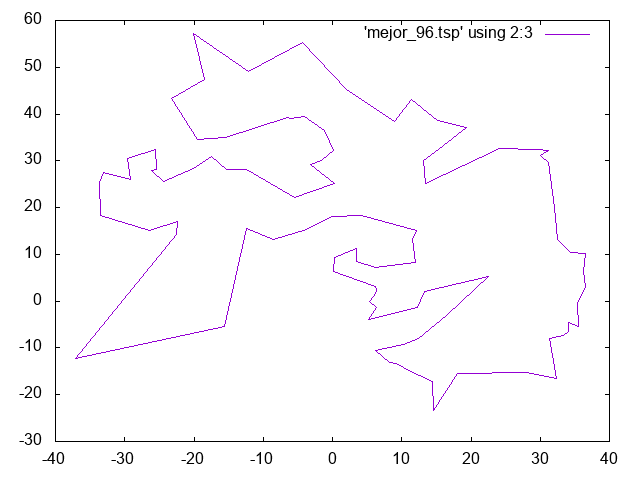
\includegraphics[width=\textwidth]{gr96_mejor.png}
\caption{Versión óptima}
\end{subfigure}
\caption{\textit{gr96.tsp}}
\end{figure}
%%%%%%%%%%%%%%%%%%%%%%%%%%%%
\begin{figure}[H]
\centering
\begin{subfigure}[b]{0.36\textwidth}
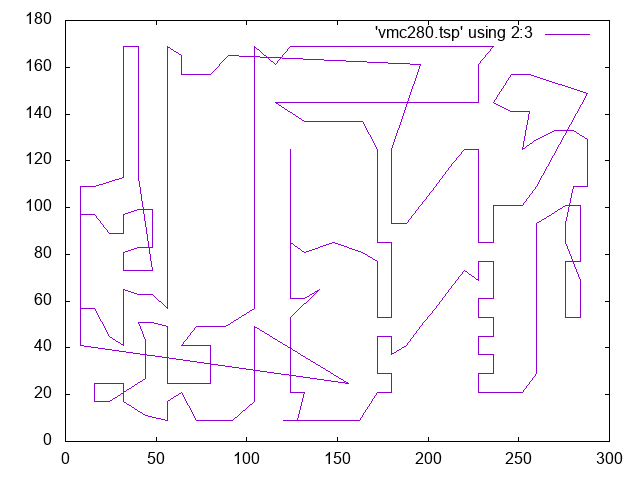
\includegraphics[width=\textwidth]{a280_vmc.png}
\caption{Vecino más cercano}
\end{subfigure}
\quad
\begin{subfigure}[b]{0.36\textwidth}
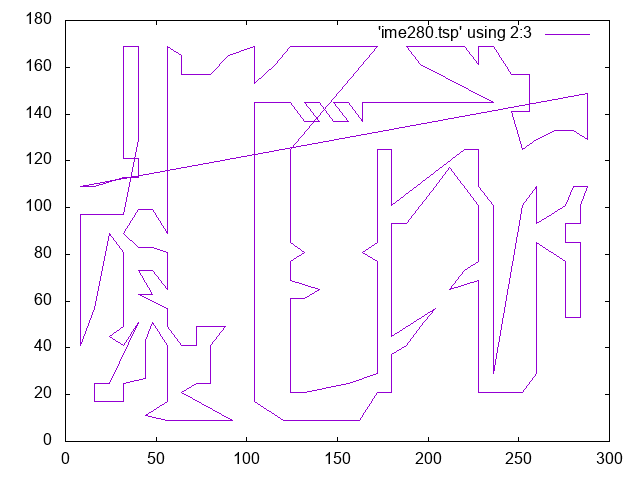
\includegraphics[width=\textwidth]{a280_ime.png}
\caption{Inserción más económica}
\end{subfigure}

\vspace{1cm}

\begin{subfigure}[b]{0.36\textwidth}
%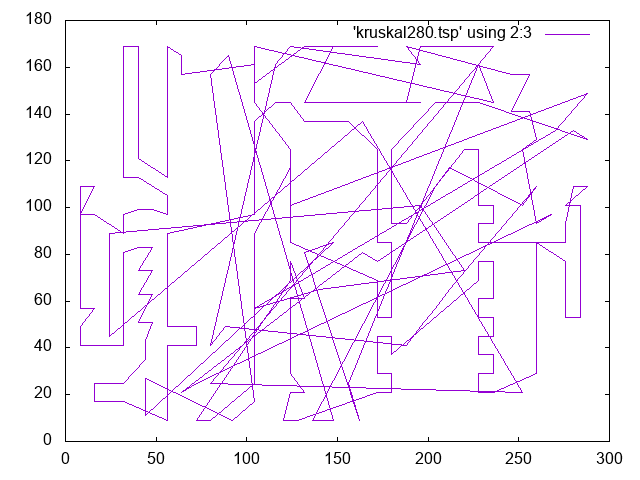
\includegraphics[width=\textwidth]{a280_kruskal.png}
\caption{Derivado de Kruskal}
\end{subfigure}
\quad
\begin{subfigure}[b]{0.36\textwidth}
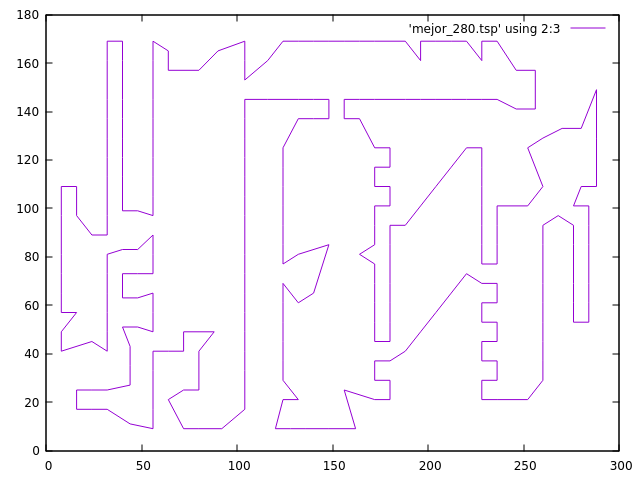
\includegraphics[width=\textwidth]{a280_mejor.png}
\caption{Versión óptima}
\end{subfigure}
\caption{\textit{a280.tsp}}
\end{figure}
%%%%%%%%%%%%%%%%%%%%%%%%%%
\begin{figure}[H]
\centering
\begin{subfigure}[b]{0.36\textwidth}
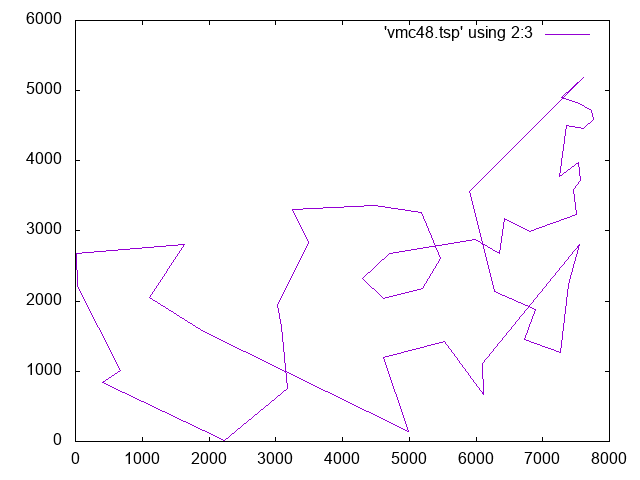
\includegraphics[width=\textwidth]{att48_vmc.png}
\caption{Vecino más cercano}
\end{subfigure}
\quad
\begin{subfigure}[b]{0.36\textwidth}
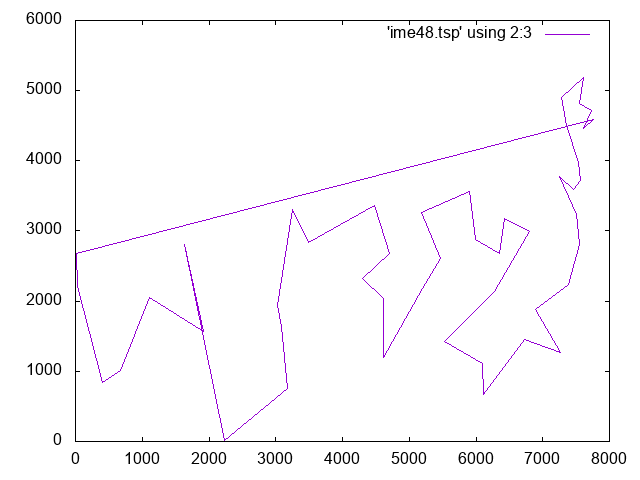
\includegraphics[width=\textwidth]{att48_ime.png}
\caption{Inserción más económica}
\end{subfigure}

\vspace{1cm}

\begin{subfigure}[b]{0.36\textwidth}
%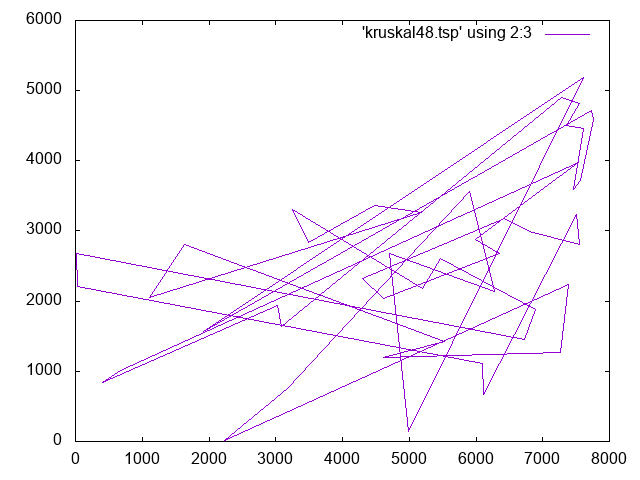
\includegraphics[width=\textwidth]{att48_kruskal.png}
\caption{Derivado de Kruskal}
\end{subfigure}
\quad
\begin{subfigure}[b]{0.36\textwidth}
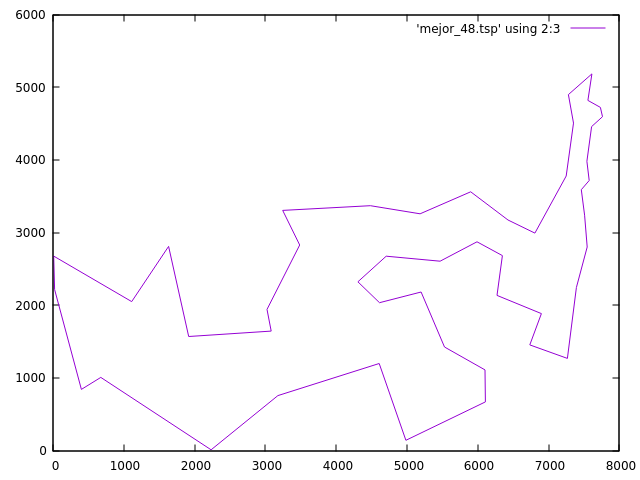
\includegraphics[width=\textwidth]{att48_mejor.png}
\caption{Versión óptima}
\end{subfigure}
\caption{\textit{att48.tsp}}
\end{figure}

%%%%%%%%%%%%%%%%%%%%%%%%%%
\begin{figure}[H]
\centering
\begin{subfigure}[b]{0.36\textwidth}
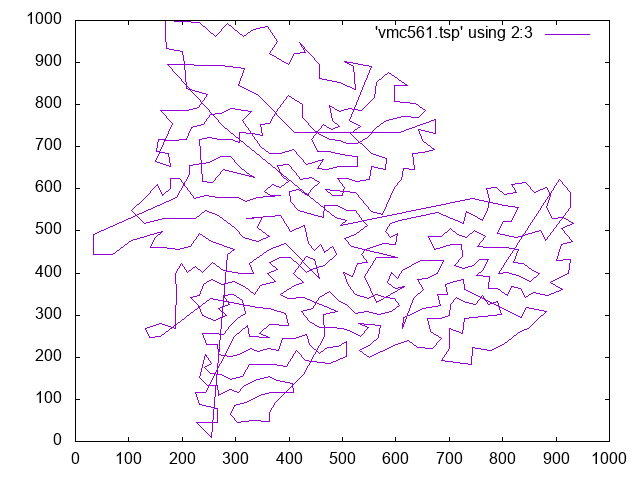
\includegraphics[width=\textwidth]{pa561_vmc.png}
\caption{Vecino más cercano}
\end{subfigure}
\quad
\begin{subfigure}[b]{0.36\textwidth}
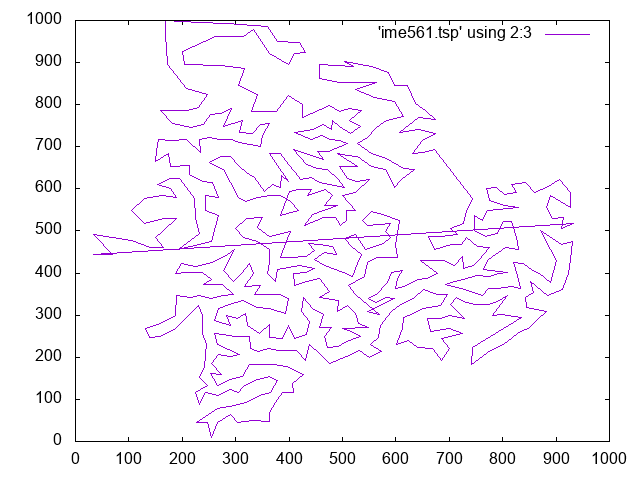
\includegraphics[width=\textwidth]{pa561_ime.png}
\caption{Inserción más económica}
\end{subfigure}

\vspace{1cm}

\begin{subfigure}[b]{0.36\textwidth}
%\includegraphics[width=\textwidth]{pa561_kruskal.png}
\caption{Derivado de Kruskal}
\end{subfigure}
\quad
\begin{subfigure}[b]{0.36\textwidth}
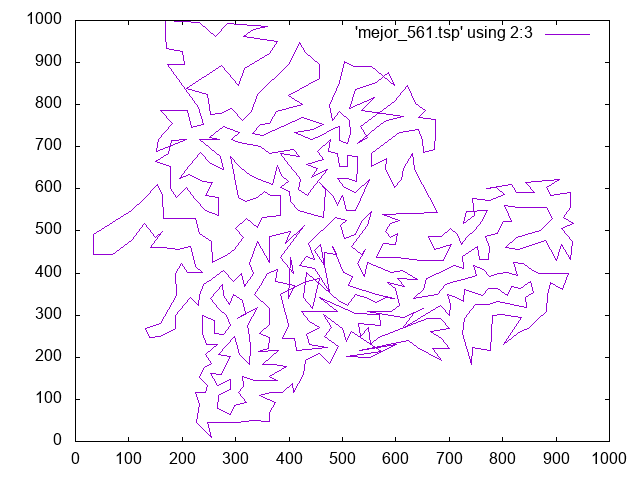
\includegraphics[width=\textwidth]{pa561_mejor.png}
\caption{Versión óptima}
\end{subfigure}
\caption{\textit{pa561.tsp}}
\end{figure}

%%%%%%%%%%%%%%%%%%%%%%%%%%
\begin{figure}[H]
\centering
\begin{subfigure}[b]{0.36\textwidth}
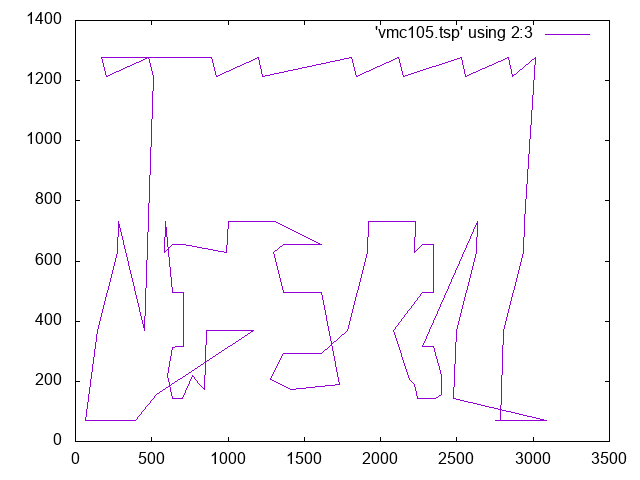
\includegraphics[width=\textwidth]{lin105_vmc.png}
\caption{Vecino más cercano}
\end{subfigure}
\quad
\begin{subfigure}[b]{0.36\textwidth}
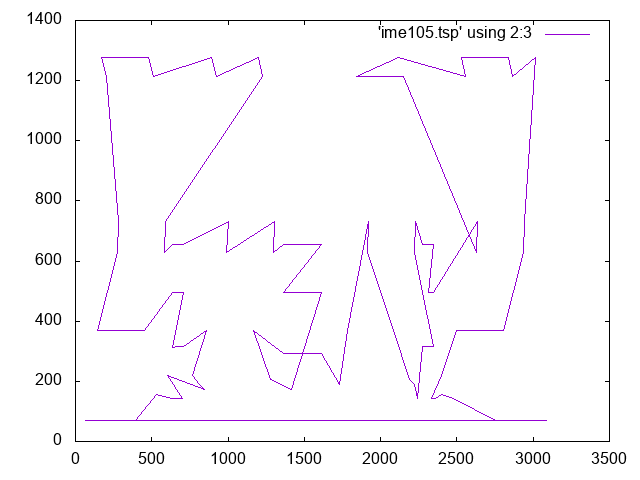
\includegraphics[width=\textwidth]{lin105_ime.png}
\caption{Inserción más económica}
\end{subfigure}

\vspace{1cm}

\begin{subfigure}[b]{0.36\textwidth}
%\includegraphics[width=\textwidth]{lin105_kruskal.png}
\caption{Derivado de Kruskal}
\end{subfigure}
\quad
\begin{subfigure}[b]{0.36\textwidth}
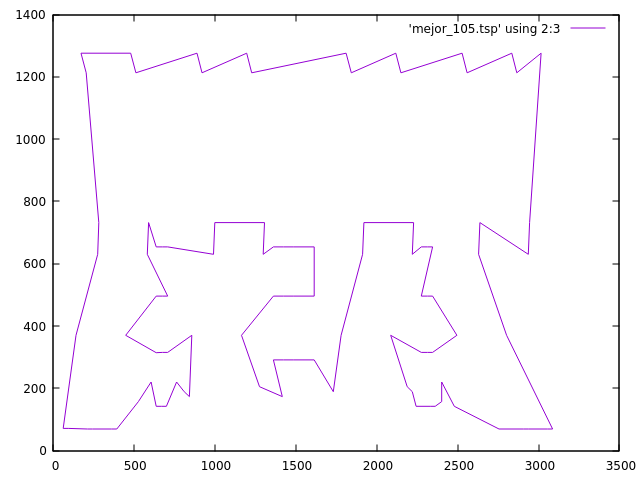
\includegraphics[width=\textwidth]{lin105_mejor.png}
\caption{Versión óptima}
\end{subfigure}
\caption{\textit{lin105.tsp}}
\end{figure}
%%%%%%%%%%%%%%%%%%%%%%%%%%
\begin{figure}[H]
\centering
\begin{subfigure}[b]{0.36\textwidth}
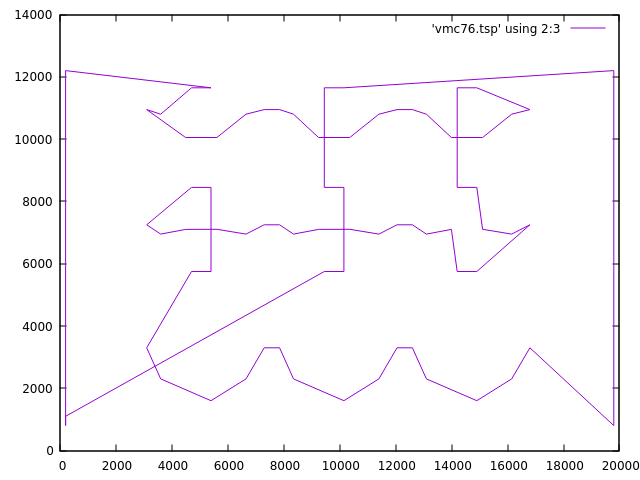
\includegraphics[width=\textwidth]{pr76_vmc.png}
\caption{Vecino más cercano}
\end{subfigure}
\quad
\begin{subfigure}[b]{0.36\textwidth}
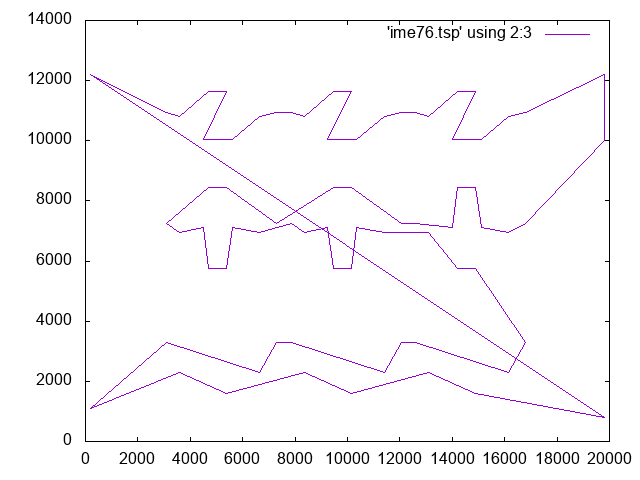
\includegraphics[width=\textwidth]{pr76_ime.png}
\caption{Inserción más económica}
\end{subfigure}

\vspace{1cm}

\begin{subfigure}[b]{0.36\textwidth}
%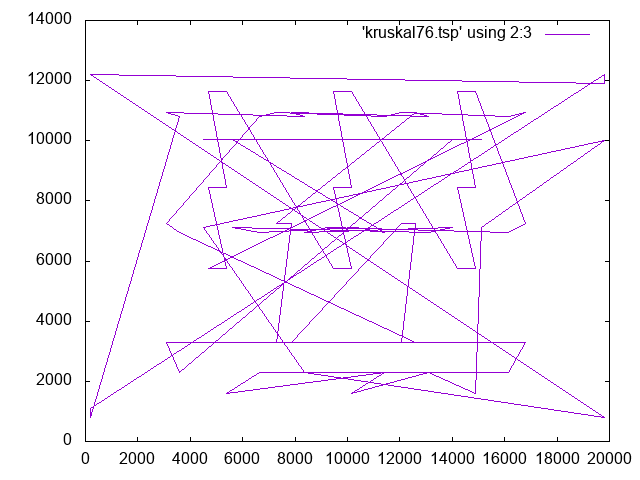
\includegraphics[width=\textwidth]{pr76_kruskal.png}
\caption{Derivado de Kruskal}
\end{subfigure}
\quad
\begin{subfigure}[b]{0.36\textwidth}
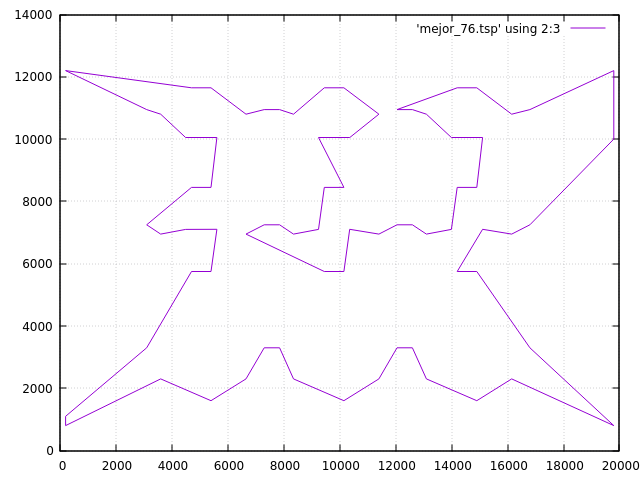
\includegraphics[width=\textwidth]{pr76_mejor.png}
\caption{Versión óptima}
\end{subfigure}
\caption{\textit{pr76.tsp}}
\end{figure}

%%%%%%%%%%%%%%%%%%%%%%%%%%
\begin{figure}[H]
\centering
\begin{subfigure}[b]{0.36\textwidth}
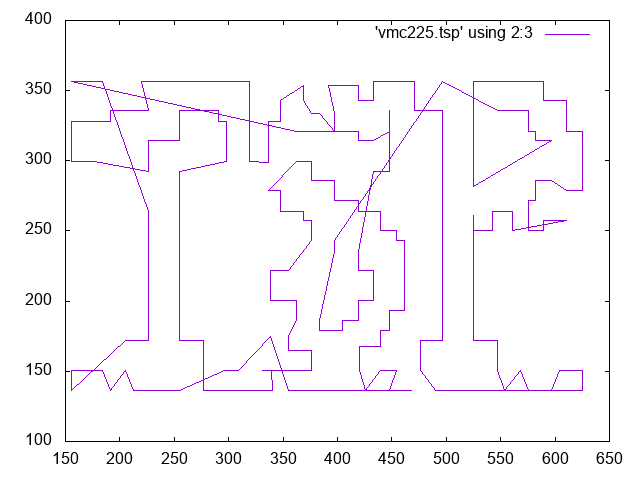
\includegraphics[width=\textwidth]{tsp225_vmc.png}
\caption{Vecino más cercano}
\end{subfigure}
\quad
\begin{subfigure}[b]{0.36\textwidth}
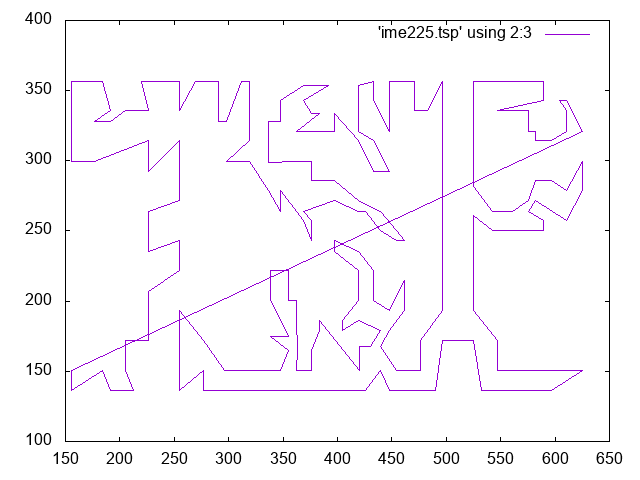
\includegraphics[width=\textwidth]{tsp225_ime.png}
\caption{Inserción más económica}
\end{subfigure}

\vspace{1cm}

\begin{subfigure}[b]{0.36\textwidth}
%\includegraphics[width=\textwidth]{tsp225_kruskal.png}
\caption{Derivado de Kruskal}
\end{subfigure}
\quad
\begin{subfigure}[b]{0.36\textwidth}
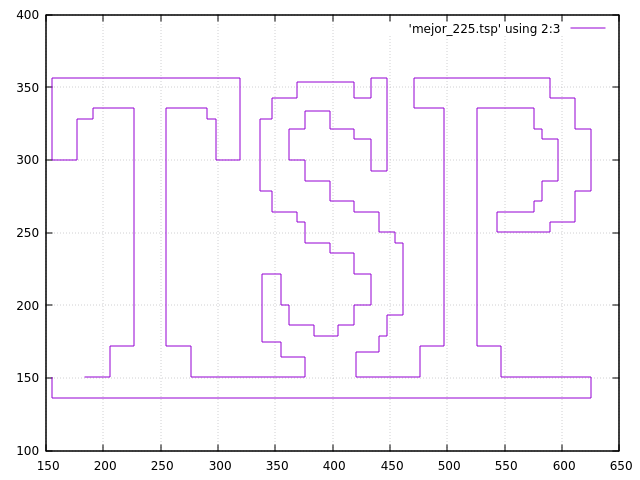
\includegraphics[width=\textwidth]{tsp225_mejor.png}
\caption{Versión óptima}
\end{subfigure}
\caption{\textit{tsp225.tsp}}
\end{figure}

%%%%%%%%%%%%%%%%%%%%%%%%%%
\begin{figure}[H]
\centering
\begin{subfigure}[b]{0.36\textwidth}
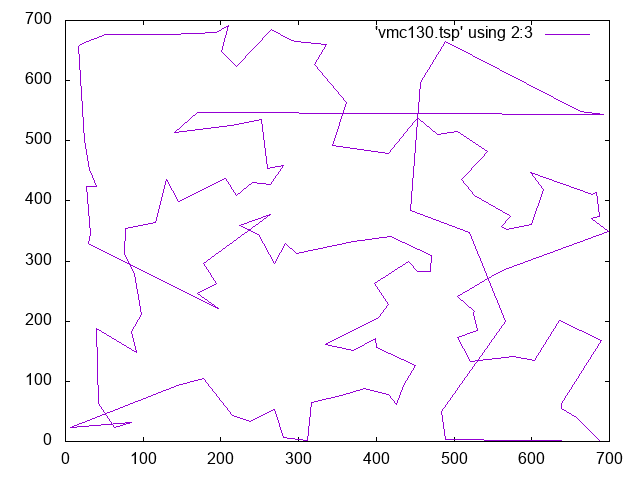
\includegraphics[width=\textwidth]{ch130_vmc.png}
\caption{Vecino más cercano}
\end{subfigure}
\quad
\begin{subfigure}[b]{0.36\textwidth}
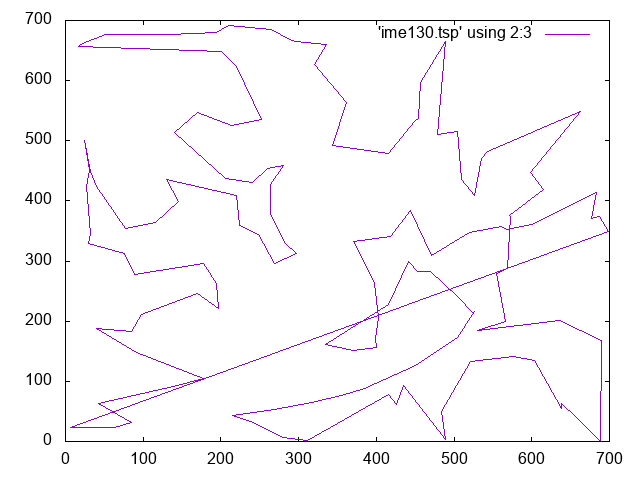
\includegraphics[width=\textwidth]{ch130_ime.png}
\caption{Inserción más económica}
\end{subfigure}

\vspace{1cm}

\begin{subfigure}[b]{0.36\textwidth}
%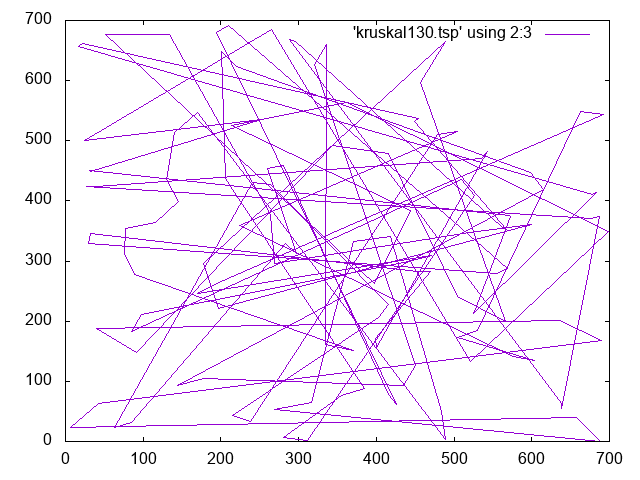
\includegraphics[width=\textwidth]{ch130_kruskal.png}
\caption{Derivado de Kruskal}
\end{subfigure}
\quad
\begin{subfigure}[b]{0.36\textwidth}
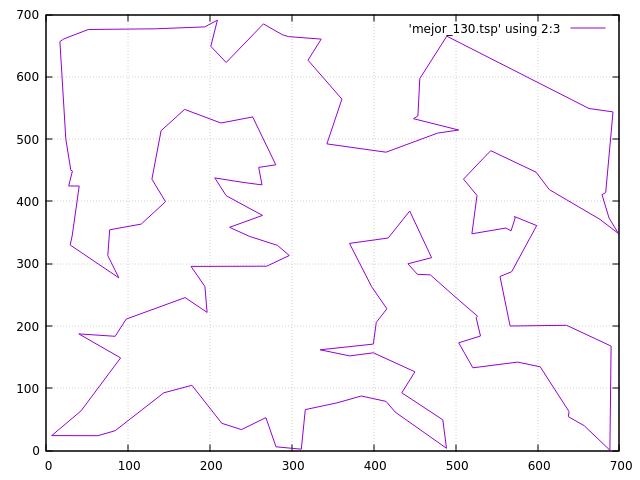
\includegraphics[width=\textwidth]{ch130_mejor.png}
\caption{Versión óptima}
\end{subfigure}
\caption{\textit{ch130.tsp}}
\end{figure}

%%%%%%%%%%%%%%%%%%%%%%%%%%
\begin{figure}[H]
\centering
\begin{subfigure}[b]{0.36\textwidth}
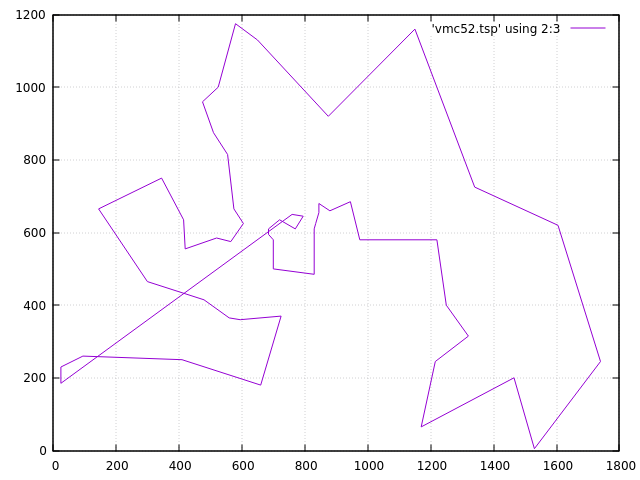
\includegraphics[width=\textwidth]{berlin52_vmc.png}
\caption{Vecino más cercano}
\end{subfigure}
\quad
\begin{subfigure}[b]{0.36\textwidth}
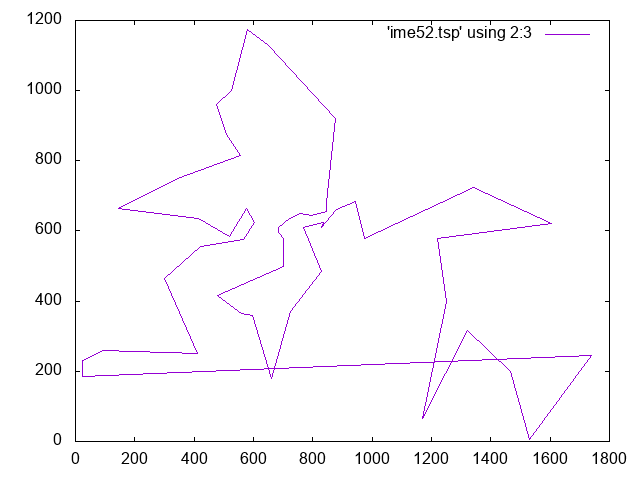
\includegraphics[width=\textwidth]{berlin52_ime.png}
\caption{Inserción más económica}
\end{subfigure}

\vspace{1cm}

\begin{subfigure}[b]{0.36\textwidth}
%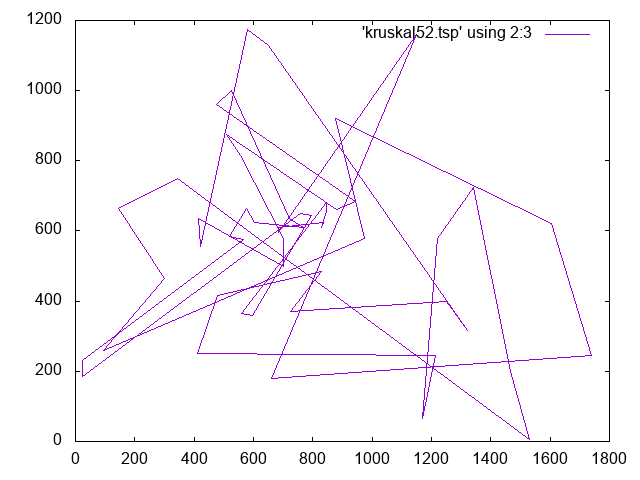
\includegraphics[width=\textwidth]{berlin52_kruskal.png}
\caption{Derivado de Kruskal}
\end{subfigure}
\quad
\begin{subfigure}[b]{0.36\textwidth}
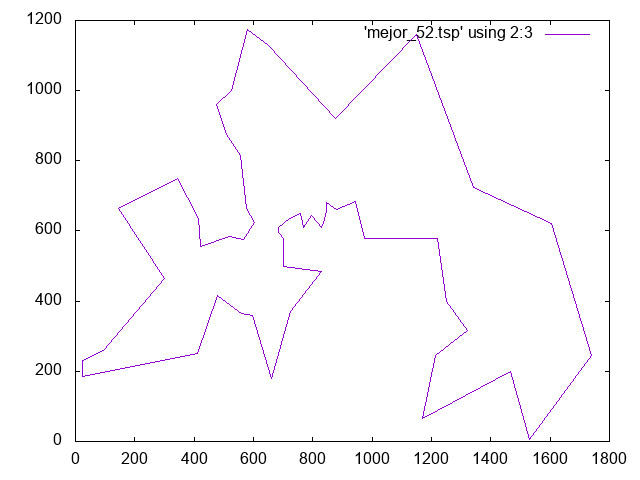
\includegraphics[width=\textwidth]{berlin52_mejor.png}
\caption{Versión óptima}
\end{subfigure}
\caption{\textit{berlin52.tsp}}
\end{figure}

%%%%%%%%%%%%%%%%%%%%%%%%%%
\begin{figure}[H]
\centering
\begin{subfigure}[b]{0.36\textwidth}
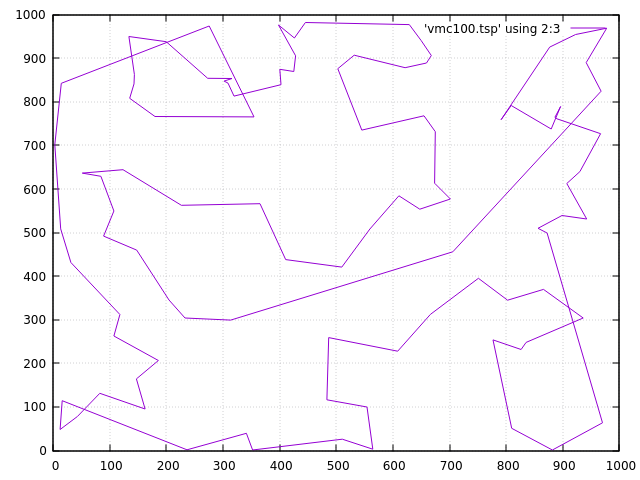
\includegraphics[width=\textwidth]{rd100_vmc.png}
\caption{Vecino más cercano}
\end{subfigure}
\quad
\begin{subfigure}[b]{0.36\textwidth}
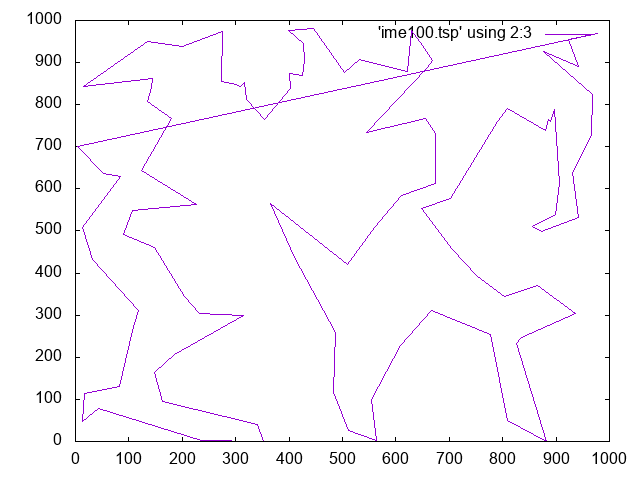
\includegraphics[width=\textwidth]{rd100_ime.png}
\caption{Inserción más económica}
\end{subfigure}

\vspace{1cm}

\begin{subfigure}[b]{0.36\textwidth}
%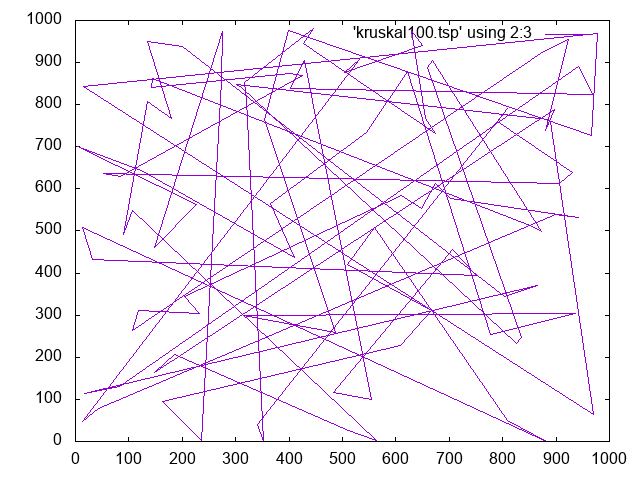
\includegraphics[width=\textwidth]{rd100_kruskal.png}
\caption{Derivado de Kruskal}
\end{subfigure}
\quad
\begin{subfigure}[b]{0.36\textwidth}
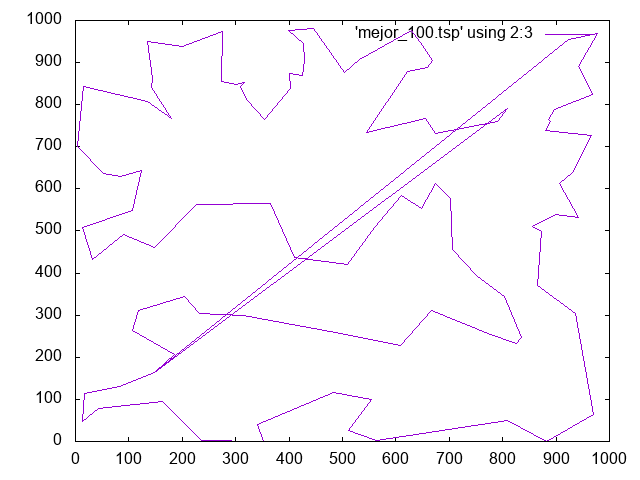
\includegraphics[width=\textwidth]{rd100_mejor.png}
\caption{Versión óptima}
\end{subfigure}
\caption{\textit{rd100.tsp}}
\end{figure}

%%%%%%%%%%%%%%%%%%%%%%%%%%
\begin{figure}[H]
\centering
\begin{subfigure}[b]{0.36\textwidth}
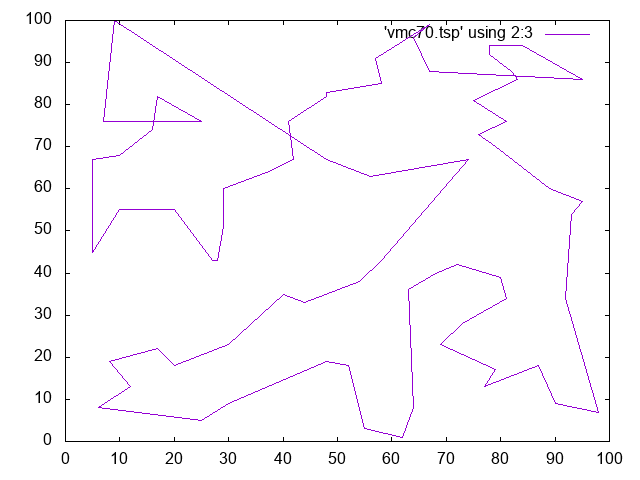
\includegraphics[width=\textwidth]{st70_vmc.png}
\caption{Vecino más cercano}
\end{subfigure}
\quad
\begin{subfigure}[b]{0.36\textwidth}
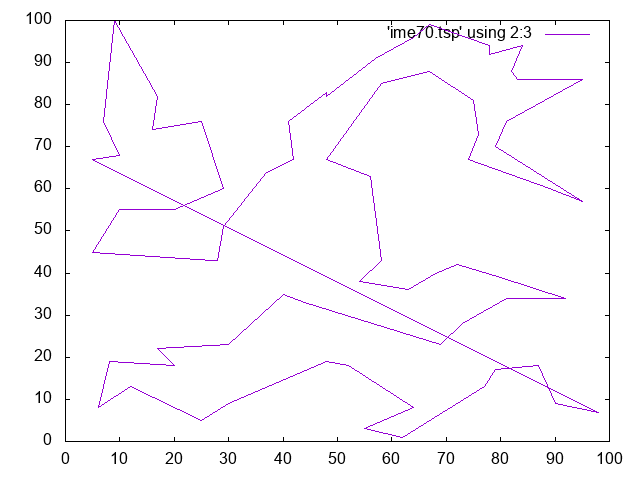
\includegraphics[width=\textwidth]{st70_ime.png}
\caption{Inserción más económica}
\end{subfigure}

\vspace{1cm}

\begin{subfigure}[b]{0.36\textwidth}
%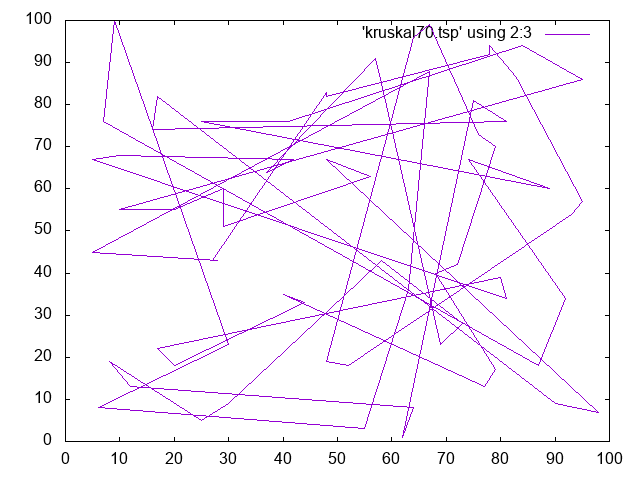
\includegraphics[width=\textwidth]{st70_kruskal.png}
\caption{Derivado de Kruskal}
\end{subfigure}
\quad
\begin{subfigure}[b]{0.36\textwidth}
\includegraphics[width=\textwidth]{st70_mejor.png}
\caption{Versión óptima}
\end{subfigure}
\caption{\textit{st70.tsp}}
\end{figure}
\newpage
\section{Anexo: código fuente}

\cppcode{tsp.cpp}
\captionof{figure}{Programa que calcula el orden según las distintas heurísticas}

\cppcode{calcular_distancia.cpp}
\captionof{figure}{Programa que calcula la distancia del circuito a partir de un fichero con coordenadas y una lista ordenada de ciudades con sus respectivas coordenadas.}

\script{ejecucion_mejor_opcion.sh}
\captionof{figure}{Script que genera archivos de coordenadas a partir de la mejor opción dada como lista.}

\script{ejecucion_tres_heuristicas.sh}
\captionof{figure}{Script que genera archivos de coordenadas a partir de las tres heurísticas desarrolladas.}

\script{gnuplot.sh}
\captionof{figure}{Script que genera las gráficas de los problemas a partir de archivos de coordenadas.}

\script{practica.sh}
\captionof{figure}{Script genera todo lo necesario para la práctica.}

%%%%%%%%%%%%%%%%%%%%%%%%%%%%Fin del documento%%%%%%%%%%%%%%%%%%%%%%%%%%%%%%%%
\end{document}
